\subsection{Preimilinares}

\begin{itemize}
    \item \textbf{Oficina del profesor}: 310 - 404
    \item \textbf{Libros}:
    \begin{itemize}
        \item \textit{Notes in General Topology} --- Hatcher
        \item \textit{Topology} --- Jänich
        \item \textit{Topology: An Exercise Textbook} --- Viro, Ivanov
    \end{itemize}
    \item \textbf{Evaluación}:
    \begin{itemize}
        \item 2 exámenes del 25\% cada uno
        \item 1 examen final del 30\%
        \item Quices cada dos semanas del 20\%
    \end{itemize}
\end{itemize}

\subsection{Topología}

Una definición importante para el concepto es el de función continua, la cual tradicionalmente se define como:

\[
\begin{aligned}
f: \mathbb{R}^n &\longrightarrow \mathbb{R}^m \\
x &\longmapsto f(x)
\end{aligned}
\]

Se dice que $f$ es continua en $x_0$ si para todo $\epsilon > 0$ existe un $\delta > 0$ tal que:

\[
\forall x \in \mathbb{R}^n, \quad \|x - x_0\| < \delta \implies \|f(x) - f(x_0)\| < \epsilon
\]

\subsection{Espacios Topológicos}

\textbf{Definición}: Sea $U \subseteq \mathbb{R}$, $U$ es abierto si para todo $x \in U$ existe un $\delta>0$ tal que:
\begin{align*}
    B_\delta(x) = \{y \in \mathbb{R} : |y - x| < \delta\} \subseteq U
\end{align*}
\begin{center}
    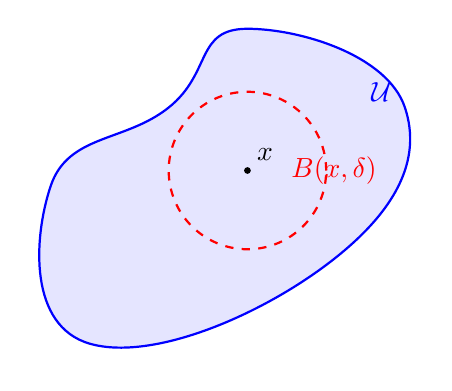
\begin{tikzpicture}
      % Draw the open set as a smooth closed curve
      \fill[blue!10] plot [smooth cycle, tension=0.8] coordinates {(0,0) (3,1) (4,3) (2,4) (1,3) (-0.5,2)}; 
      \draw[blue, thick] plot [smooth cycle, tension=0.8] coordinates {(0,0) (3,1) (4,3) (2,4) (1,3) (-0.5,2)};
    
      % Label the open set
      \node[blue] at (3.7,3.2) {$\mathcal{U}$};
    
      % Point x inside the set
      \filldraw[black] (2,2.2) circle (1pt) node[above right] {$x$};
    
      % Open ball around x with radius delta
      \draw[red, dashed, thick] (2,2.2) circle (1cm);
      \node[red] at (3.1,2.2) {$B(x,\delta)$};
    \end{tikzpicture}
\end{center}

\textbf{Propiedades}:

\begin{itemize}
    \item $U$ es abierto sii $\operatorname{Int}(U) = U (x \in \operatorname{Int}(U) \text{ si } \exists \delta > 0: B_\delta(x) \subseteq U)$
    \item $\{U_i\}_{i \in I}$ es una \textbf{una familia de cojuntos abiertos} entonces:
    \begin{align*}
        \bigcup_{i \in I} U_i &\text{ es abierto} \\
    \end{align*}
    \item Si $U_1, U_2, \dots, U_n$ son abiertos entonces:
    \begin{align*}
        U_1 \cap U_2 \cap \dots \cap U_n &\text{ es abierto} \\
    \end{align*}
\end{itemize}
\textbf{Demostración}: Ejercicio (Considere $\emptyset$ y $\mathbb{R}$ como abiertos)

\textbf{Definición (Espacio topológico)}: Un espacio topológico es una tupla $(X, \mathcal{T})$ donde $X$ es un conjunto y $\mathcal{T}$ es una familia de subconjuntos abiertos $X$ que satisfacen:
\begin{enumerate}
    \item $\emptyset, X \in \mathcal{T}$.
    \item Si $\{U_i\}_{i \in I} \subseteq \mathcal{T}$ entonces
    \begin{align*}
        \bigcup_{i \in I} U_i &\in \mathcal{T}
    \end{align*}
    Es decir $\mathcal {T}$ es cerrado bajo uniones arbitrarias de subconjuntos abiertos de $X$.
    \item Si $U_1, U_2, \dots, U_n \in \mathcal{T}$ entonces
    \begin{align*}
        U_1 \cap U_2 \cap \dots \cap U_n &\in \mathcal{T}
    \end{align*}
    Es decir $\mathcal {T}$ es cerrado bajo intersecciones finitas de subconjuntos abiertos de $X$.
\end{enumerate}
\textbf{Ejemplo}: Consideremos $\{B_\epsilon(x): \epsilon > 0\}$ con $x$ fijo. Entonces $\bigcap_{\epsilon>0} B_{\epsilon}(x) = \{x\}$ no es abierto.

\textbf{Ejercicios (Hatcher)}: Pagina 14,15, ejercicios 1 y 13.

\subsubsection{Continuidad}

\textbf{Definición Continuidad en $\mathbb{R}$}: Sea $f: \mathbb{R}^n \to \mathbb{R}^m$ una función. Decimos que $f$ si para todo $\epsilon > 0$ y para todo $x \in X$, la vecindad abierta $B_\epsilon(f(x))$ tiene una vecindad abierta $B_\delta(x)$ tal que $f(B_\delta(x)) \subseteq B_\epsilon(f(x))$.

\textbf{Definición topológica de continuidad:} Dados dos espacios topológicos $(X, \mathcal{T}_X)$ y $(Y, \mathcal{T}_Y)$, decimos que una función $f:X \mapsto Y$ es continua si, para todo $x \in X$ y para todo abierto $V \in \mathcal{T}_Y$ tal que $f(x) \in V$, existe un abierto $U \in \mathcal{T}_X$ que satisface que $x \in U$ y $f(U) \subseteq V$.

\textbf{Proposición}: Una función $f: X \to Y$ es continua si y solo si para todo conjunto abierto $V \subseteq Y$ se cumple que $f^{-1}(V) \in \mathcal{T}_X$ es abierta.

\textbf{Demostración 1}:
\begin{itemize}
    \item \textbf{($\implies$)}: Sea $V \subseteq f(X)$:
        %% Diagram of X, Y, f(X) and V
        \begin{center}
            \shorthandoff{>}
        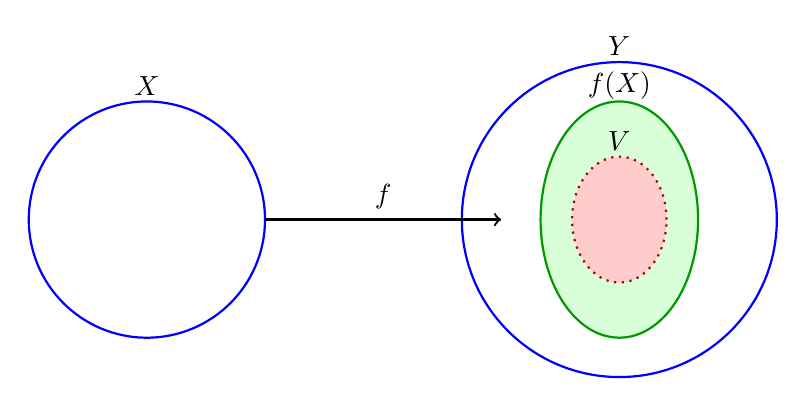
\begin{tikzpicture}[scale=1]
            % Set X
            \draw[blue, thick] (-3,0) circle (1.5cm);
            \node at (-3,1.7) {$X$};

            % Set Y
            \draw[blue, thick] (3,0) circle (2cm);
            \node at (3,2.2) {$Y$};

            % Arrow representing the function f
            \draw[->, thick] (-1.5,0) -- (1.5,0) node[midway, above] {\(f\)};

            % Image f(X) inside Y
            \fill[green!15] (3,0) ellipse (1cm and 1.5cm);
            \draw[green!60!black, thick] (3,0) ellipse (1cm and 1.5cm);
            \node at (3,1.7) {$f(X)$};

            % Subset V inside f(X)
            \fill[red!20] (3,0.0) ellipse (0.6cm and 0.8cm);
            \draw[red!70!black, thick, dotted] (3,0.0) ellipse (0.6cm and 0.8cm);
            \node at (3,1.0) {$V$};
        \end{tikzpicture}
        \shorthandon{>}
        \end{center}
    
    Para ver que $f^{-1}(V)$ es abierto, consideremos $x \in f^{-1}(V)$. Entonces existe $y \in V$ tal que $f(x) = y$. Como $V$ es abierto, existe una vecindad abierta $\mathcal M_y$ tal que $y\in \mathcal M_y \subseteq V$. 

    \begin{center}
        \shorthandoff{>}
        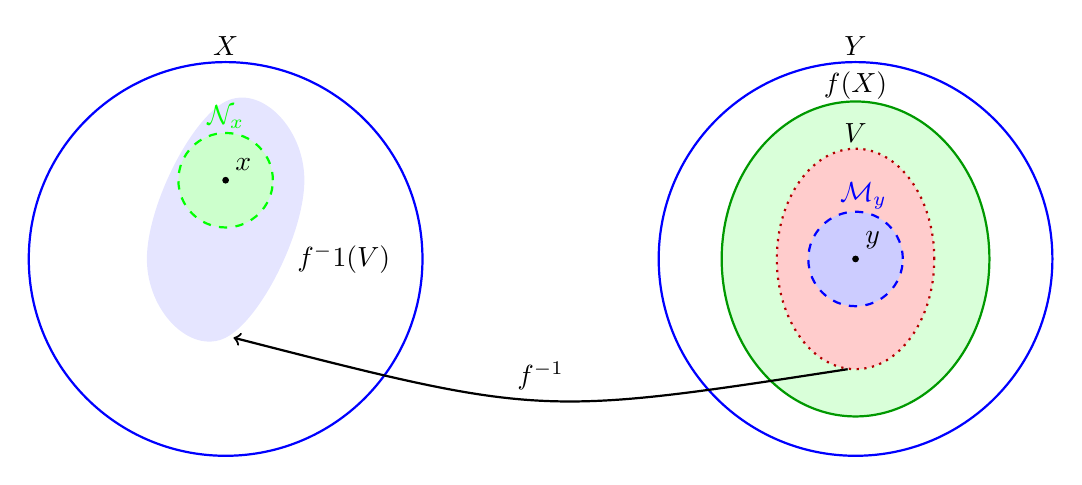
\begin{tikzpicture}
            % Set x
             \draw[blue, thick] (-4,0) circle (2.5cm);
             \node at (-4,2.7) {$X$};

            % Draw the set U in X
            \node at (-2.5,0) {$f^-{1}(V)$};
            \fill[blue!10] plot [smooth cycle, tension=0.8] coordinates {(-5,0) (-4,-1) (-3,1) (-4,2)};

            % Neighborhood of x
            \fill[green!20] (-4,1.0)  circle (.6cm);
            \filldraw[black] (-4,1) circle (1pt) node[above right] {$x$};
            \draw[green, dashed, thick] (-4,1) circle (.6cm);
            \node[green!100] at (-4,1.8) {$\mathcal{N}_x$};


             % Set Y
             \draw[blue, thick] (4,0) circle (2.5cm);
             \node at (4,2.7) {$Y$};
 
             % Image f(X) inside Y
             \fill[green!15] (4,0) ellipse (1.7cm and 2.0cm);
             \draw[green!60!black, thick] (4,0) ellipse (1.7cm and 2.0cm);
             \node at (4,2.2) {$f(X)$};
 
             % Subset V inside f(X)
             \fill[red!20] (4,0.0) ellipse (1.0cm and 1.4cm);
             \draw[red!70!black, thick, dotted] (4,0.0) ellipse (1.0cm and 1.4cm);
             \node at (4,1.6) {$V$};

            % Arc arrow representing the function f^-1 from V to U
            \draw[->, thick] (3.9,-1.4) .. controls (0,-2) .. (-3.9,-1) node[midway, above] {\(f^{-1}\)};


            %point y and neighborhood radius epsilon
            \fill[blue!20] (4,0.0)  circle (.6cm);
            \filldraw[black] (4,0) circle (1pt) node[above right] {$y$};
            \draw[blue, dashed, thick] (4,0) circle (.6cm);
            \node[blue] at (4.1,.8) {$\mathcal M_y$};
        \end{tikzpicture}
        \shorthandon{>}
    \end{center}

    Ahora por la definición de continuidad para $x \in X$  y para $\mathcal M_y$ existe una vecindad abierta $\mathcal N_x \subseteq X$ tal que $x \in \mathcal N_x$ y $f(\mathcal N_x) \subseteq \mathcal M_y \subseteq V$. 

    \begin{center}
        \shorthandoff{>}
        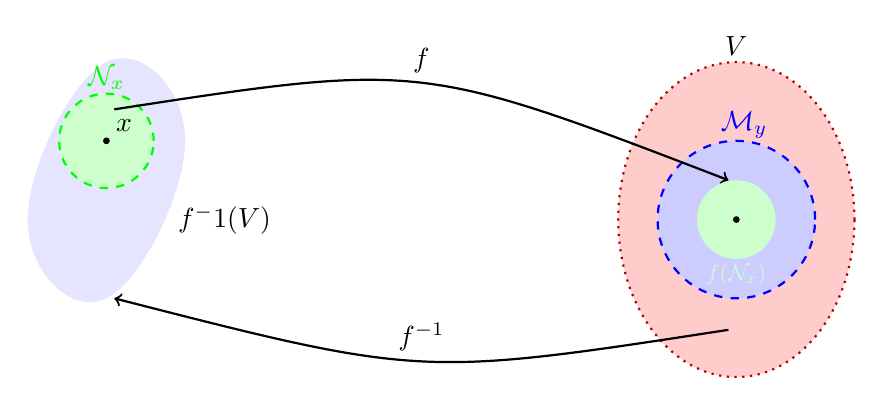
\begin{tikzpicture}

            % Draw the set U in X
            \node at (-2.5,0) {$f^-{1}(V)$};
            \fill[blue!10] plot [smooth cycle, tension=0.8] coordinates {(-5,0) (-4,-1) (-3,1) (-4,2)};

            % Neighborhood of x
            \fill[green!20] (-4,1.0)  circle (.6cm);
            \filldraw[black] (-4,1) circle (1pt) node[above right] {$x$};
            \draw[green, dashed, thick] (-4,1) circle (.6cm);
            \node[green!100] at (-4,1.8) {$\mathcal{N}_x$};


             % Subset V inside f(X)
             \fill[red!20] (4,0.0) ellipse (1.5cm and 2cm);
             \draw[red!70!black, thick, dotted] (4,0.0) ellipse (1.5cm and 2cm);
             \node at (4,2.2) {$V$};

            % Arc arrow representing the function f^-1 from V to U
            \draw[->, thick] (3.9,-1.4) .. controls (0,-2) .. (-3.9,-1) node[midway, above] {\(f^{-1}\)};


            %point y and neighborhood radius epsilon
            \fill[blue!20] (4,0.0)  circle (1cm);
            \filldraw[black] (4,0) circle (1pt) node[above right] {$y$};
            \draw[blue, dashed, thick] (4,0) circle (1cm);
            \node[blue] at (4.1,1.2) {$\mathcal M_y$};

            % Arrow from x N_x to y M_y
            \draw[->, thick] (-3.9,1.4) .. controls (0,2) .. (3.9,.5) node[midway, above] {\(f\)};

            % f(N_x) subset of M_y
            \fill[green!20] (4,0.0)  circle (.5cm);
            \filldraw[black] (4,0) circle (1pt);
            \node[green!20,scale=0.8] at (4,-.7) {$f(\mathcal{N}_x)$};
        \end{tikzpicture}
        \shorthandon{>}
    \end{center}
    

    Asi por la definición de imagen $f^{-1}(V) = \{ x \in X : f(x) \in V\}$, $\mathcal N_x \subseteq f^{-1}(V)$, pues todos $x' \in \mathcal N_x$ cumplen que $f(x') \in f(\mathcal N_x) \subseteq \mathcal M_y \subseteq V$. Asi para cualquier $x \in f^{-1}(V)$ existe una vecindad abierta $\mathcal N_x$ tal que $x \in \mathcal N_x$ y $f(\mathcal N_x) \subseteq V$. Por lo tanto $f^{-1}(V)$ es abierto.
    
    \item \textbf{($\impliedby$)}: Sea $x \in X$ y $y = f(x) \in f(X) \subseteq Y$, y supongamos que existe que existe $\in V \subseteq^{ab} f(X)$, pues en otro caso se cumple por vacuidad. Entonces por hipótesis $f^{-1}(V)$ es abierto.
    \begin{center}
        \shorthandoff{>}
        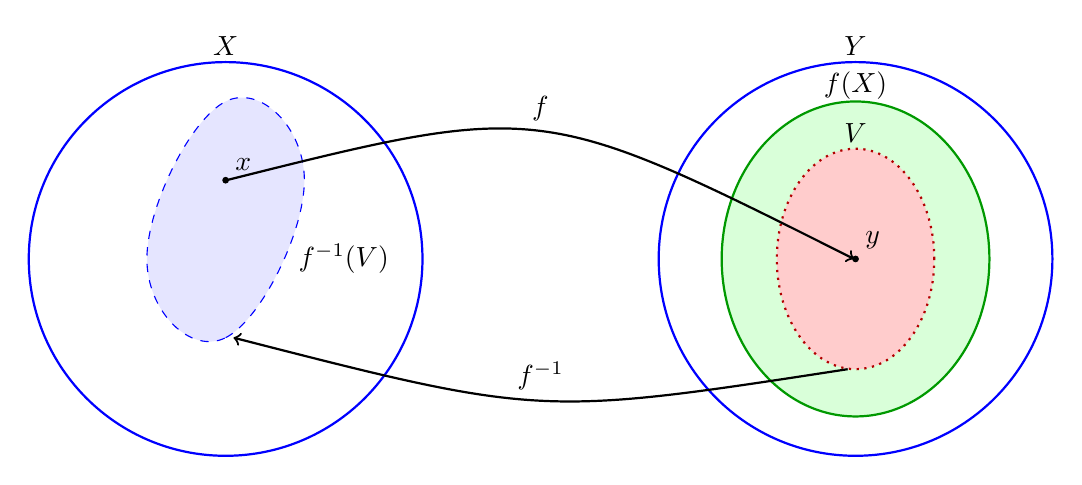
\begin{tikzpicture}
            % Set x
             \draw[blue, thick] (-4,0) circle (2.5cm);
             \node at (-4,2.7) {$X$};

            % Draw the set U in X
            \node at (-2.5,0) {$f^{-1}(V)$};
            \fill[blue!10] plot [smooth cycle, tension=0.8] coordinates {(-5,0) (-4,-1) (-3,1) (-4,2)};
            \draw[blue, dashed] plot [smooth cycle, tension=0.8] coordinates {(-5,0) (-4,-1) (-3,1) (-4,2)};        % Set Y
             \draw[blue, thick] (4,0) circle (2.5cm);

            % Point x inside the set
            \filldraw[black] (-4,1) circle (1pt) node[above right] {$x$};


            % Set Y
             \node at (4,2.7) {$Y$};
             % Image f(X) inside Y
             \fill[green!15] (4,0) ellipse (1.7cm and 2.0cm);
             \draw[green!60!black, thick] (4,0) ellipse (1.7cm and 2.0cm);
             \node at (4,2.2) {$f(X)$};
 
             % Subset V inside f(X)
             \fill[red!20] (4,0.0) ellipse (1.0cm and 1.4cm);
             \draw[red!70!black, thick, dotted] (4,0.0) ellipse (1.0cm and 1.4cm);
             \node at (4,1.6) {$V$};

             % Point y in V
            \filldraw[black] (4,0) circle (1pt) node[above right] {$y$}; 

            % Arrow from x to y

            \draw[->, thick] (-3.99,1) .. controls (0,2) .. (3.98,0) node[midway, above] {\(f\)};

            % Arc arrow representing the function f^-1 from V to U
            \draw[->, thick] (3.9,-1.4) .. controls (0,-2) .. (-3.9,-1) node[midway, above] {\(f^{-1}\)};

        \end{tikzpicture}
        \shorthandon{>}
    \end{center}

    Luego para todo $x \in X$ y para todo $V \in \mathcal{T}_Y$ tal que $f(x) \in V$, existe una vecindad abierta $f^{-1}(V)$ tal que $x \in f^{-1}(V)$ y $f(f^{-1}(V)) \subseteq V$. Por lo tanto $f$ es continua.
\end{itemize}

De este modo podemos realizar la siguiente definición:

\textbf{Definición Continuidad 2}: Sea $f: X \to Y$ (donde $X$ y $Y$ son espacios topológicos) es continua si la imagen inversa bajo $f$ de abiertos en $Y$ son abiertos en $X$.

\subsubsection{Ejemplos de espacios topológicos}

En $\mathbb{R}$ podemos definir los siguientes espacios topológicos:
\begin{itemize}
    \item \textbf{Topología trivial}: $\mathcal{T}_t = \{\emptyset, \mathbb{R}\}$
    \item \textbf{Topología discreta}: $\mathcal{T}_d = \mathscr P(\mathbb{R})$. En esta topología los singletons son abiertos, y por lo tanto, cualquier conjunto es abierto.
    \item \textbf{Topología de complementos finitos (topología de Zariski)}: $\mathcal{T}_f = \{U \subseteq \mathbb{R} : U = \emptyset \text{ o } U^c \text{ es finito}\}$. En esta topología los conjuntos abiertos son aquellos cuyo complemento es finito, es muy importante en \textit{geometría algebraica}.
    \item \textbf{Topología de cerrado-abierto}: $\mathcal{T}_{ca} = \{U \subseteq \mathbb{R} : \forall x \in U, \exists a,b \in \mathbb R \text{ tal que } x \in [a,b) \subseteq U\}$. En esta topología los conjuntos abiertos son aquellos que contienen intervalos semi-abiertos de la forma $[a,b)$. La topología usual $\mathcal{T}_u$ seria $\mathcal{T}_{aa}$.
\end{itemize}

\textbf{Dem $\mathcal T_z$ es topología}: 
Verifiquemos que cumple las propiedades de la definición de topología:
\begin{enumerate}
    \item $\emptyset \in \mathcal{T}_z$  por definición.
    \item $\mathbb{R} \in \mathcal{T}_z$, pues $\mathbb{R}^c = \emptyset$ es finito.
    \item Sea $\{U_i\}_{i \in I} \subseteq \mathcal{T}_z$ y $U = \bigcup_{i \in I} U_i$. Entonces:
    \begin{align*}
        U^c &= \left(\bigcup_{i \in I} U_i\right)^c = \bigcap_{i \in I} U_i^c
    \end{align*}
    Con $U_i^c$ finito por hipótesis.
    \begin{itemize}
        \item si $U^c = \emptyset$ entonces $U \in \mathcal{T}_z$.
        \item si $U^c \neq \emptyset$, si por contradicción $U^c$ es infinito y dado que $U^c \subseteq U_i^c$ para todo $i \in I$, entonces $U_i^c$ es infinito, lo cual contradice la hipótesis de que $U_i^c$ es finito. Por lo tanto $U^c$ es finito y $U \in \mathcal{T}_z$.
    \end{itemize}
    \item Sea $U_1, U_2, \dots, U_n \in \mathcal{T}_z$ y $U = U_1 \cap U_2 \cap \dots \cap U_n$. Entonces:
    \begin{align*}
        U^c &= (U_1 \cap U_2 \cap \dots \cap U_n)^c = \bigcup_{i=1}^n U_i^c
    \end{align*}
    Con $U_i^c$ finito por hipótesis, por lo que $U^c$ es la union finita de conjuntos finitos, por lo tanto $U^c$ es finito. Por lo tanto $U \in \mathcal{T}_z$.
\end{enumerate}
Por lo tanto $\mathcal{T}_z$ es una topología sobre $\mathbb{R}$.

\textbf{Ejercicio}: Verificar que $\mathcal{T}_{ca}$ es una topología sobre $\mathbb{R}$.

\textbf{Diagrama de Hasse}

Tenemos 6 \textbf{topologias} en \( \mathbb{R} \), relacionadas entre si por la contenencia de la siguiente manera:

\begin{align*}
    \mathscr{T}_t \subseteq \mathscr{T}_z \subseteq \mathscr{T}_{cont} & \subseteq \mathscr{T}_d \\
    \mathscr{T}_z \subseteq \mathscr{T}_u \subseteq \mathscr{T}_{ca} \subseteq \mathscr{T}_d
\end{align*}

Lo cual se puede representar en el siguiente diagrama de Hasse:

\begin{center}
\shorthandoff{>}
\begin{tikzpicture}[>=latex]
  \node (Tt) at (0,0) {$\mathscr{T}_t$};
  \node (Tz) at (0,1.5) {$\mathscr{T}_z$};
  \node (Tcont) at (-1.5,3) {$\mathscr{T}_{cont}$};
  \node (Tu) at (1.5,3) {$\mathscr{T}_u$};
  \node (Td) at (0,6) {$\mathscr{T}_d$};
  \node (Tca) at (1.5,4.5) {$\mathscr{T}_{ca}$};
  \draw (Tt) -- (Tz) -- (Tcont);
  \draw (Tcont) -- (Td);
  \draw (Tz) -- (Tu) -- (Tca);
  \draw (Tca) -- (Td);
\end{tikzpicture}
\shorthandon{>}
\end{center}

\textbf{Nota:} La topología $\mathscr{T}_{\text{cont}}$ la topología de los complementos contables.